\documentclass[tikz,border=2pt]{standalone}
\usepackage{amsmath}
\usepackage{amssymb}
\usepackage{pgfplots}
\pgfplotsset{compat=1.18}
\usetikzlibrary{arrows.meta}
\begin{document}
% Left (m=2): Cone({(1,0),(1,1)}) is the sector 0<=x2<=x1; (1,2)=-v1+2v2 is not in it.
% Right (m=3): Cone({(1,0),(0,1),(-1,-1)}) is all of R^2; (-3,1)=3v3+4v2.
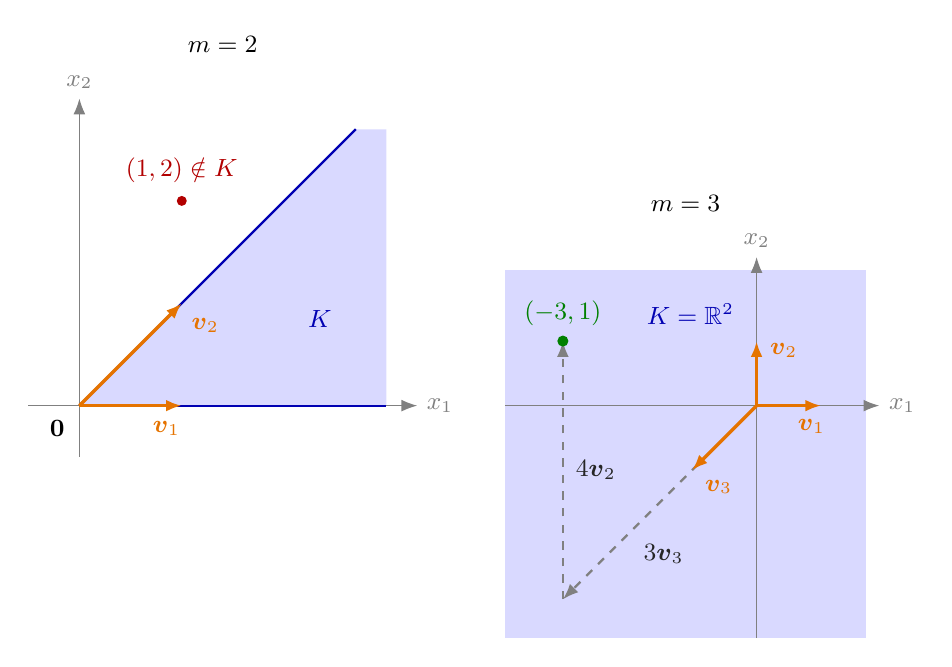
\begin{tikzpicture}[font=\small, >={Latex[length=2mm]}]
  % ---------- left panel: two generators
  \begin{scope}[x=1.3cm, y=1.3cm]
    \fill[blue!15] (0,0) -- (3,0) -- (3,2.7) -- (2.7,2.7) -- cycle;
    \draw[gray, ->] (-0.5,0) -- (3.3,0) node[anchor=west] {$x_1$};
    \draw[gray, ->] (0,-0.5) -- (0,3.0) node[anchor=south] {$x_2$};
    \draw[blue!70!black, thick] (0,0) -- (3,0);
    \draw[blue!70!black, thick] (0,0) -- (2.7,2.7);
    \draw[orange!90!black, very thick, ->] (0,0) -- (1,0);
    \draw[orange!90!black, very thick, ->] (0,0) -- (1,1);
    \node[orange!90!black, anchor=north] at (0.85,-0.06) {$\boldsymbol{v}_1$};
    \node[orange!90!black, anchor=north west] at (1.0,0.95) {$\boldsymbol{v}_2$};
    \node[blue!70!black] at (2.35,0.85) {$K$};
    \fill[red!70!black] (1,2) circle (1.8pt);
    \node[red!70!black, anchor=south] at (1,2.08) {$(1,2)\notin K$};
    \node[anchor=north east] at (-0.05,-0.05) {$\boldsymbol{0}$};
    \node[anchor=south] at (1.4,3.35) {$m=2$};
  \end{scope}
  % ---------- right panel: three generators fill the plane
  \begin{scope}[xshift=8.6cm, x=0.82cm, y=0.82cm]
    \fill[blue!15] (-3.9,-3.6) rectangle (1.7,2.1);
    \draw[gray, ->] (-3.9,0) -- (1.9,0) node[anchor=west] {$x_1$};
    \draw[gray, ->] (0,-3.6) -- (0,2.3) node[anchor=south] {$x_2$};
    \draw[gray, thick, dashed, ->] (0,0) -- (-3,-3);
    \draw[gray, thick, dashed, ->] (-3,-3) -- (-3,1);
    \node[gray!30!black, anchor=north west] at (-1.9,-2.0) {$3\boldsymbol{v}_3$};
    \node[gray!30!black, anchor=west] at (-2.95,-1.0) {$4\boldsymbol{v}_2$};
    \draw[orange!90!black, very thick, ->] (0,0) -- (1,0);
    \draw[orange!90!black, very thick, ->] (0,0) -- (0,1);
    \draw[orange!90!black, very thick, ->] (0,0) -- (-1,-1);
    \node[orange!90!black, anchor=north] at (0.85,-0.06) {$\boldsymbol{v}_1$};
    \node[orange!90!black, anchor=west] at (0.06,0.85) {$\boldsymbol{v}_2$};
    \node[orange!90!black, anchor=north west] at (-0.95,-1.0) {$\boldsymbol{v}_3$};
    \fill[green!50!black] (-3,1) circle (2pt);
    \node[green!50!black, anchor=south] at (-3,1.08) {$(-3,1)$};
    \node[blue!70!black, anchor=south east] at (-0.2,1.1) {$K=\mathbb{R}^2$};
    \node[anchor=south] at (-1.1,2.85) {$m=3$};
  \end{scope}
\end{tikzpicture}
\end{document}
